\documentclass[11pt,english,compress]{beamer}

\usepackage[utf8]{inputenc}
\usepackage{verbatim}
\usepackage{eurosym}
\usepackage{stmaryrd}

\usepackage[compatibility=false]{caption}
\usepackage{subcaption}
\usepackage{pgfplots}

\useoutertheme[subsection=true]{smoothbars}
\useinnertheme[shadow=true]{rounded}

\usecolortheme{orchid}
\usecolortheme{whale}

\setcounter{tocdepth}{2}
\setcounter{secnumdepth}{0}

\setbeamertemplate{footline}[frame number]

\title{The Linux graphics stack, Optimus and the Nouveau driver}
\subtitle{Cooperative rendering across GPUs on Linux}
\author{Martin Peres}
\institute{Nouveau developer\\PhD student at LaBRI\\X.Org Foundation board member}

\AtBeginSection[]{
  \begin{frame}{Summary}
  \small \tableofcontents[currentsection, hideothersubsections]
  \end{frame} 
}

\begin{document}

\setbeamertemplate{navigation symbols}{}
\setbeamertemplate{footline}[frame number]

\begin{frame}[plain,noframenumbering]
	\titlepage
\end{frame}

\section{Introduction to the Linux graphics stack}
\subsection{General overview}
\begin{frame}
	\frametitle{General overview of the Linux Graphics stack}

	\begin{block}{The graphics stack before 2005}
		\begin{itemize}
			\item The X-Server provided everything:
			\begin{itemize}
				\item Modesetting (CRTC \& plane management);
				\item 2D/3D acceleration;
				\item Video rendering acceleration;
				\item Input management.
			\end{itemize}
			\item The X-Server talked to the GPU directly, as root.
		\end{itemize}
	\end{block}

	\begin{block}{The current graphics stack}
		\begin{itemize}
			\item The X-Server got split into more than 200 components:
			\begin{itemize}
				\item Privileged operations in the kernel;
				\item 2D drivers got put into different shared objects;
				\item 3D acceleration got put in mesa;
				\item The list is too long ;)
			\end{itemize}
		\end{itemize}
	\end{block}
\end{frame}

\begin{frame}
	\begin{figure}[h]
		\centering
		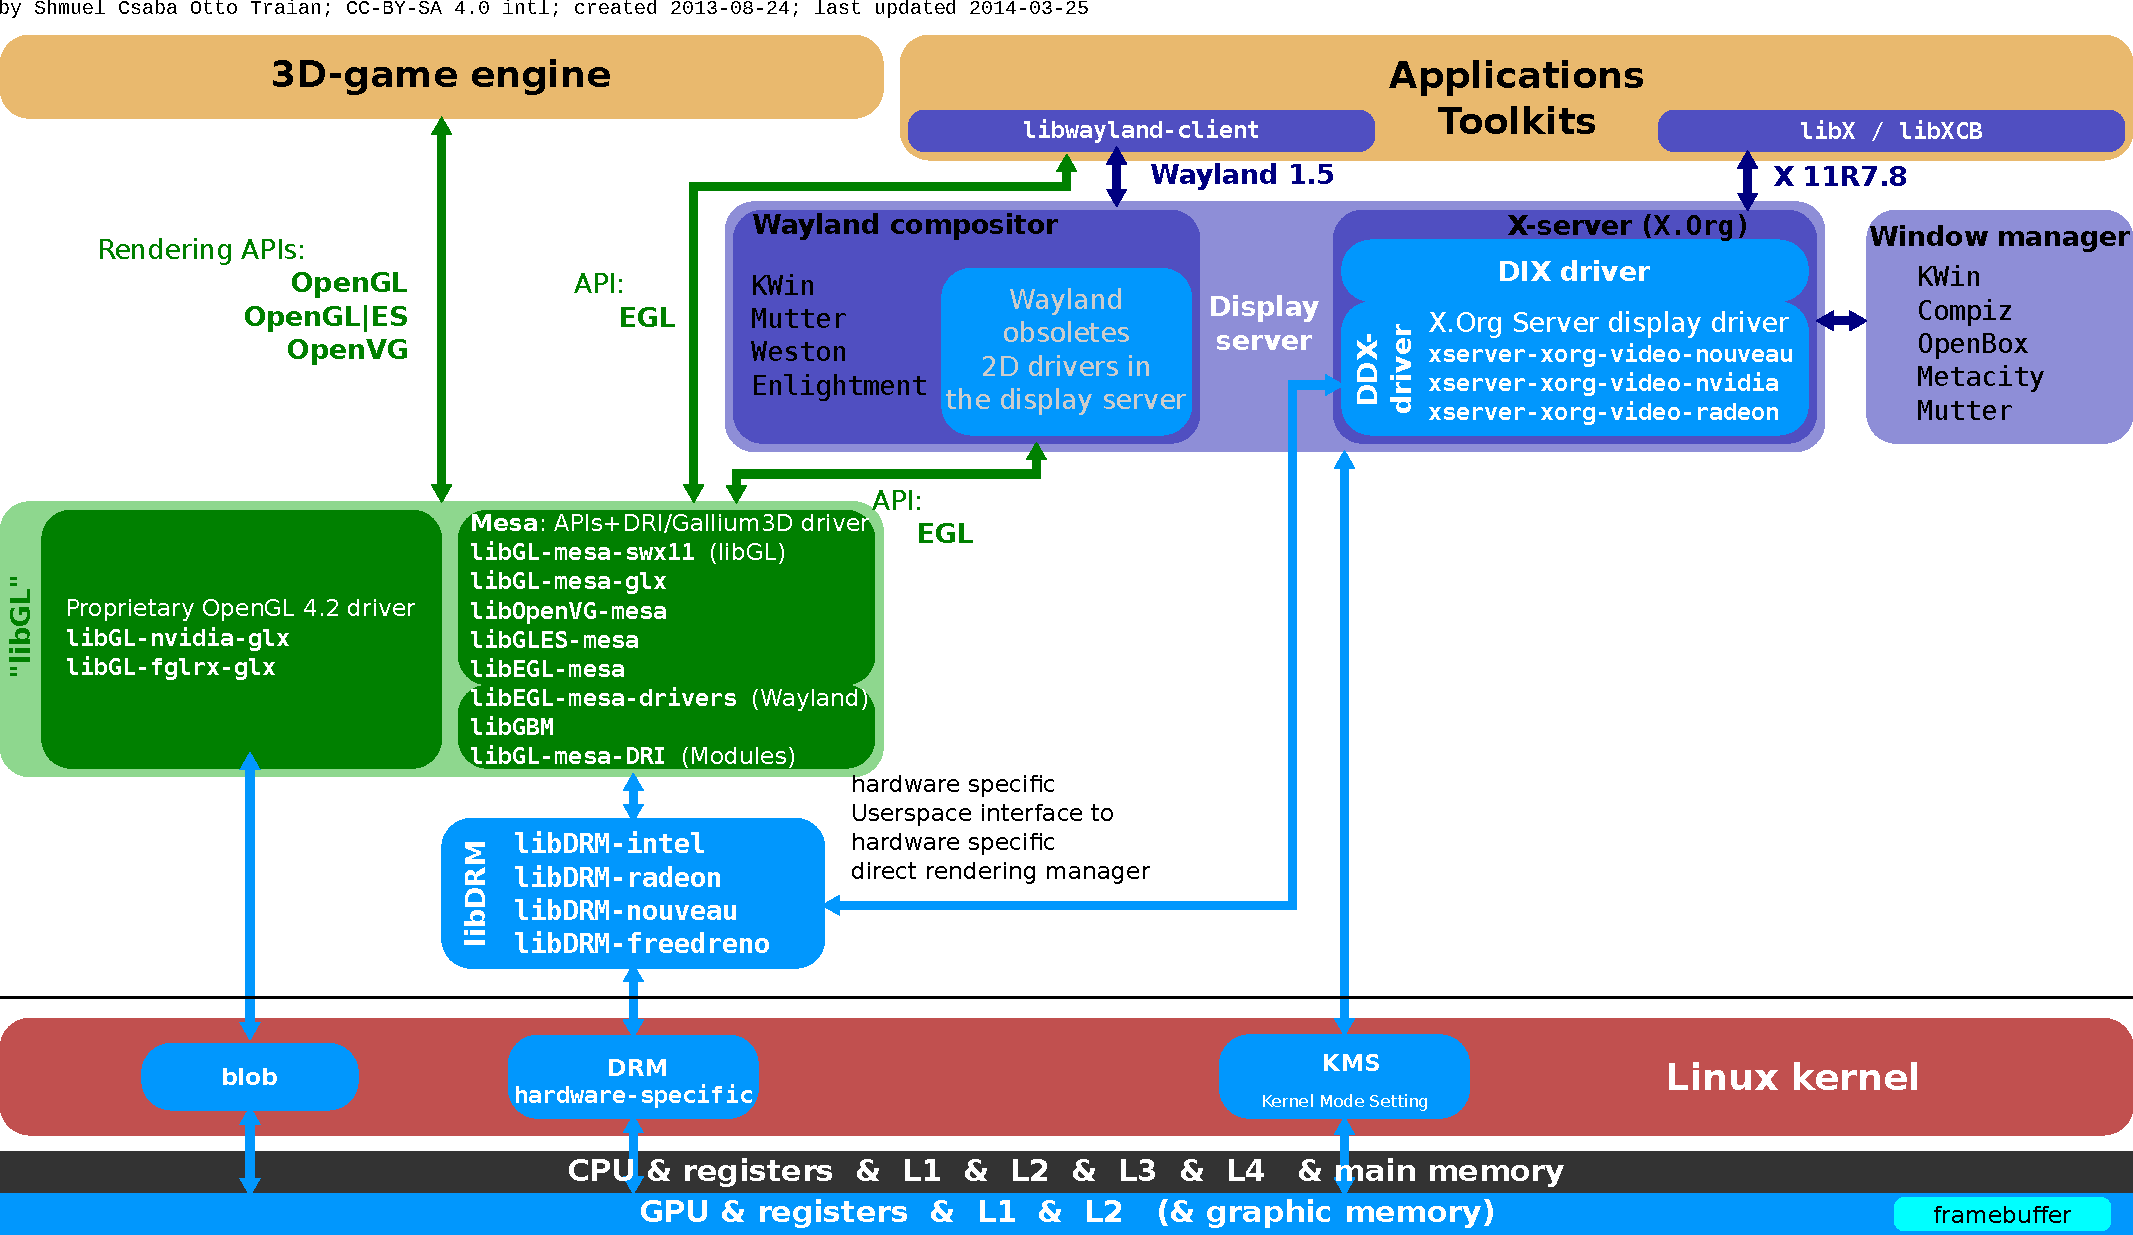
\includegraphics[width=1.02\linewidth]{imgs/Linux_Graphics_Stack_2013.pdf}
		\caption{General overview of the Linux graphics stack}
	\end{figure}
\end{frame}

\subsection{Kernel space}

\begin{frame}
	\frametitle{The kernel space}

	\begin{block}{Direct Rendering Manager (DRM) : The common code}
		\begin{itemize}
			\item This common code provides:
			\begin{itemize}
				\item Kernel ModeSetting (KMS): CRTC \& plane management;
				\item Video memory management via GEM (with a TTM backend?);
				\item Nodes with different capabilities (master or render nodes).
			\end{itemize}
		\end{itemize}
	\end{block}

	\begin{block}{DRM open source drivers}
		\begin{itemize}
			\item i810/i915: Intel;
			\item nouveau: NVIDIA;
			\item radeon: AMD/ATI;
			\item vmwgfx: VMware;
			\item many SoC GPUs (armada, exynos, msm, omap, tegra, ...).
		\end{itemize}
	\end{block}
\end{frame}

\subsection{User space}

\begin{frame}
	\frametitle{Architecture of the X-Server}

	\begin{figure}[h]
		\centering
		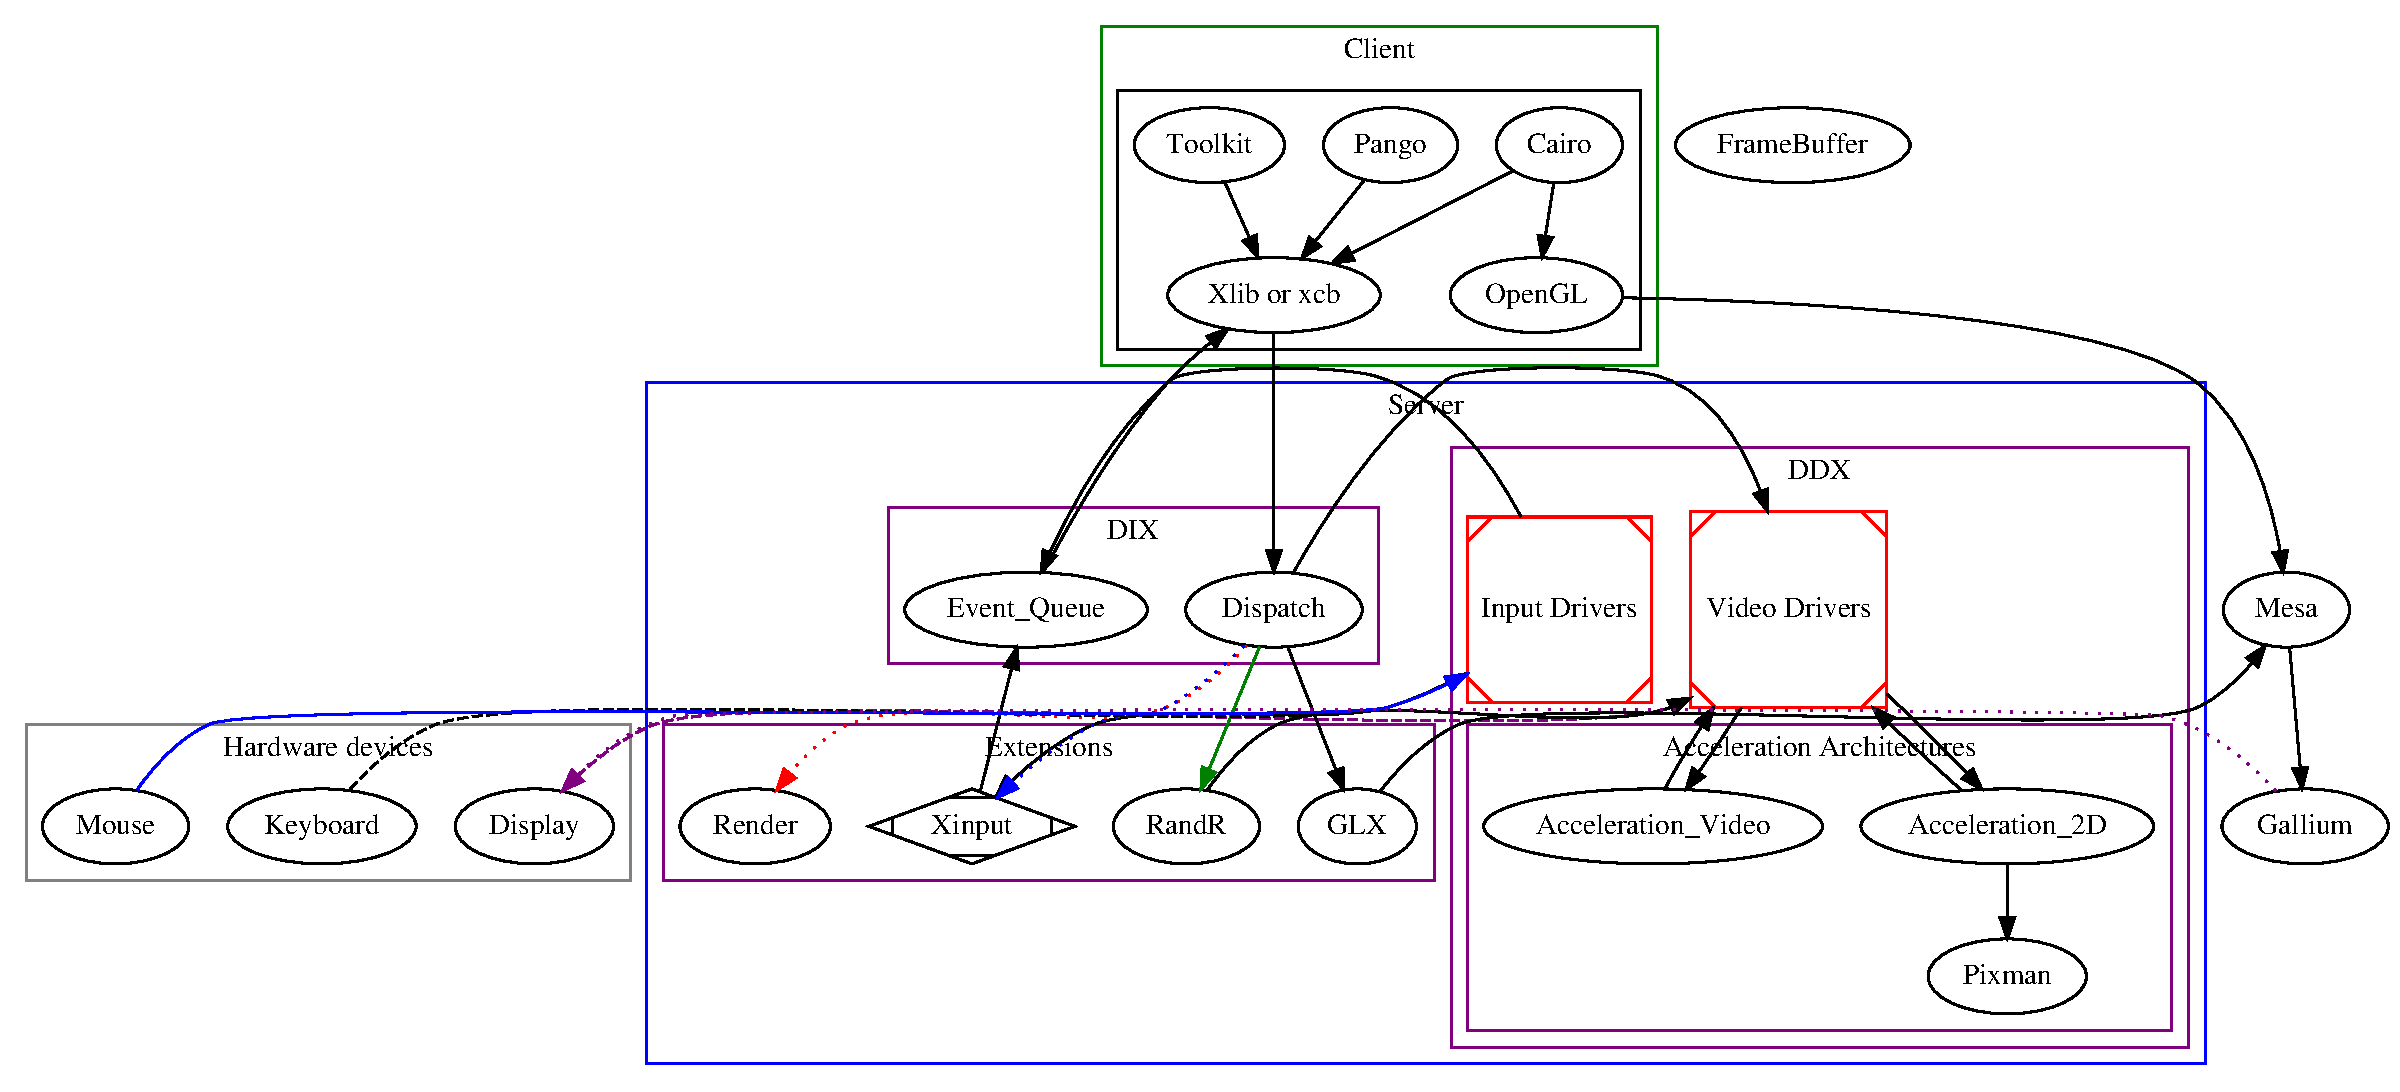
\includegraphics[width=1\linewidth]{imgs/xorg.pdf}
		\caption{General overview of the X-Server's internal architecture}
	\end{figure}
\end{frame}

\begin{frame}
	\frametitle{Architecture of Mesa}

	\begin{figure}[h]
		\centering
		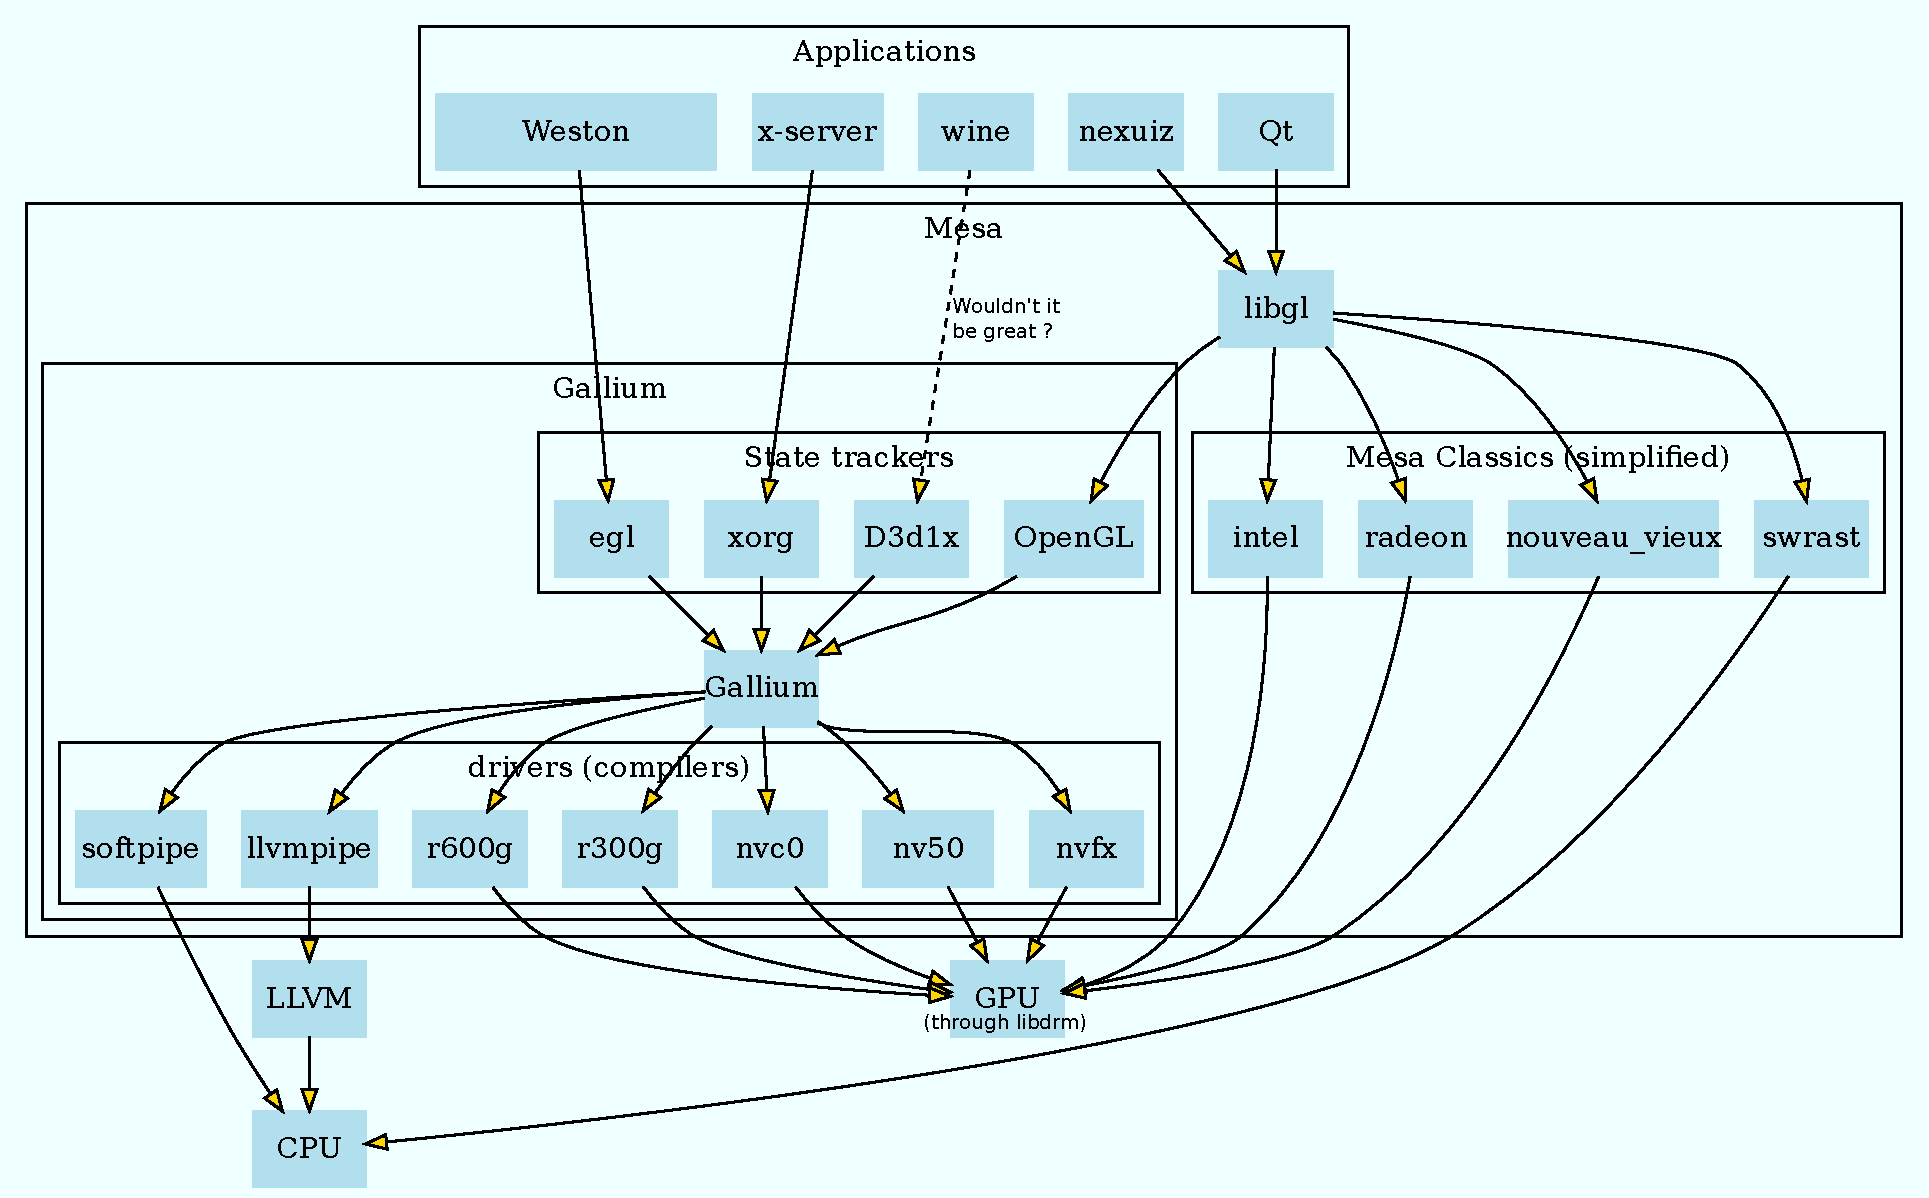
\includegraphics[width=1\linewidth]{imgs/mesa.pdf}
		\caption{General overview of Mesa's internal architecture}
	\end{figure}
\end{frame}

\section{Optimus}
\subsection{Introduction}
\begin{frame}
	\frametitle{Kepler support}

	\begin{block}{Kepler}
		\begin{itemize}
			\item New NVIDIA card family released in March 2012;
			\item Modesetting support released on the same day;
			\item Un-released 3D support happened a few days later;
			\item 2D/3D accel support released less than a month after (after libdrm2).
		\end{itemize}
	\end{block}
\end{frame}

\subsection{Introduction}

\section{Kernel}
\subsection*{Kernel updates}
\begin{frame}
	\frametitle{Kernel updates}

	\begin{block}{Kernel updates}
		\begin{itemize}
			\item Nouveau left staging (Linux 3.4);
			\item Major internal re-architecturing, called core (Linux 3.7);
		\end{itemize}
	\end{block}

	\begin{block}{The core architecture}
		\begin{itemize}
			\item Separate code per-chipset;
			\item Can partially be used from the userspace;
			\item Kind of object-oriented (ctor, dtor, init \& fini);
			\item Should limit regressions when adding support to new cards;
			\item Contribution by Ben Skeggs.
		\end{itemize}
	\end{block}
\end{frame}

% Maarten
\subsection{Optimus/prime}

\begin{frame}
	\frametitle{Optimus/prime}

	\begin{block}{Optimus/Prime support}
		\begin{itemize}
			\item Offloading support added by Dave Airlie in Linux 3.9;
			\item Synchronisation between drivers, worked on by mlankhorst;
		\end{itemize}
	\end{block}

	\begin{block}{More information + how to}
		\url{http://nouveau.freedesktop.org/wiki/Optimus/}
	\end{block}
\end{frame}

% Martin
\subsection{Power Management}

\begin{frame}
	\frametitle{Power Management}

	\begin{block}{Thermal management}
		\begin{itemize}
			\item Temperature monitoring support added for most cards;
			\item Except for the i2c-only temperature probes.
		\end{itemize}
	\end{block}

	\begin{block}{Fan management}
		\begin{itemize}
			\item Static fan management added in Linux 3.7;
			\item Experimental automatic fan management added in
Linux 3.9;
			\item Enabled by default in Linux 3.13;
			\item Doesn't work on all Keplers...
		\end{itemize}
	\end{block}

	\begin{block}{}
		Contact Martin Peres (mupuf) if you have problems!
	\end{block}
\end{frame}

\begin{frame}
	\frametitle{Power Management}

	\begin{block}{Reclocking}
		\begin{itemize}
			\item Still a work in progress...;
			\item Will provide much better performance!
		\end{itemize}
	\end{block}

	\begin{block}{Power and clock gating}
		\begin{itemize}
			\item Will lower the power consumption (good for
laptops);
			\item Should be released soon for Fermi/Kepler.
		\end{itemize}
	\end{block}

	\begin{block}{Performance and power monitoring}
		\begin{itemize}
			\item Some Kepler have i2c power sensors!
			\item Rough engine-usage indicators (Memory, Graph,
Video);
			\item Will be exposed ASAP.
		\end{itemize}
	\end{block}
\end{frame}

\section{Userspace}

\subsection{Performance counters}

\begin{frame}
	\frametitle{Performance counters}

	\begin{block}{DONE}
		\begin{itemize}
			\item MP-counters support for Fermi+;
			\item Exposed through Gallium-HUD;
			\item Kepler support by Christoph Bumiller;
			\item Fermi support by Samuel Pitoiset (GSOC 2013).
		\end{itemize}
	\end{block}

	\begin{block}{WIP}
		\begin{itemize}
			\item Performance monitoring from PDAEMON(Mem, VDec,
GR);
			\item Reverse engineering graphics-related signals on
W7 (Samuel);
			\item Export the kernels
		\end{itemize}
	\end{block}

\end{frame}

% Maarten
\subsection{Libdrm\_nouveau2}
\begin{frame}
	\frametitle{Userspace updates - Libdrm\_nouveau2}

	\begin{block}{Libdrm\_nouveau2}
		\begin{itemize}
			\item Expose BOs' VM addresses;
			\item Support multiple threads per channel;
			\item Rework the rellocation mechanism;
			\item Reduce the occurences of -ENOSPC;
			\item Released in April 2012 by Ben Skeggs.
		\end{itemize}
	\end{block}

	\begin{block}{Libdrm\_nouveau2 : Mesa updates}
		\begin{itemize}
			\item Mesa drivers updated to use Libdrm\_nouveau2;
			\item Nvfx rewritten and renamed nv30;
			\item Various fixes to the other drivers.
		\end{itemize}
	\end{block}
\end{frame}

\subsection{Video decoding}
\begin{frame}
	\frametitle{Userspace updates - Video decoding}

	\begin{block}{Video decoding : Maarten Lankhorst}
		\begin{itemize}
			\item Fermi+ support added by Maarten Lankhorst;
			\item Rely on user-extracted firmwares (mmiotrace).
		\end{itemize}
	\end{block}

	\begin{block}{Video decoding : Ilia Mirkin}
		\begin{itemize}
			\item Nv50: Full VP2/3/4 support added by Ilia Mirkin;
			\item Wrote a script to extract firmwares from the blob;
			\item Added back support for video planes on (nv04-40);
			\item PMPEG support for MPEG1/2 on nv40-96.
		\end{itemize}
	\end{block}

	\begin{block}{More information}
		\url{http://nouveau.freedesktop.org/wiki/VideoAcceleration}
	\end{block}
\end{frame}

\subsection{OpenGL}

\begin{frame}
	\frametitle{OpenGL}

	\begin{block}{History: GL version support}
		\begin{itemize}
			\item OpenGL 3.0 in Mesa 8.0 (nvc0);
			\item OpenGL 3.1 in Mesa 9 (nvc0);
			\item OpenGL 3.3 support in Mesa 10.1 for nv50/nvc0.
		\end{itemize}
	\end{block}

	\begin{block}{Limited support}
		\begin{itemize}
			\item GK110;
			\item GK208.
		\end{itemize}
	\end{block}
\end{frame}

\subsection{Direct 3D}

\begin{frame}
	\frametitle{Nine: a d3d9 state tracker}

	\begin{block}{Nine: a d3d9 state tracker}
		\begin{itemize}
			\item Started by Joakim Sindholt;
			\item Completed by Christoph Bumiller
			\item Runs Skyrim, Civilization 5, Anno 1404 and StarCraft 2;
			\item Up to 2 times faster than Wine's d3d implementation.
		\end{itemize}
	\end{block}

	\begin{block}{Announcement}
		\url{http://lists.freedesktop.org/archives/mesa-dev/2013-July/041900.html}
	\end{block}

	\begin{block}{Source tree}
		\url{https://github.com/chrisbmr/Mesa-3D/tree/gallium-nine}
	\end{block}
\end{frame}

% Marcin
\section{Tools}

\subsection{Envytools repo moved}
\begin{frame}
	\frametitle{Envytools}

	\begin{block}{Envytools}
		\begin{itemize}
			\item is a collection of nvidia-related tools and docs;
			\item was primarily hosted by Pathscale;
			\item but was also hosted by mwk \& sourceforge;
			\item moved to one repo with every dev as admins.
		\end{itemize}
	\end{block}

	\begin{block}{More information}
		\url{http://lists.freedesktop.org/archives/nouveau/2013-July/013089.html}
	\end{block}
\end{frame}

\subsection{RESTification of the documentation}
\begin{frame}
	\frametitle{Envytools : documentation}

	\begin{block}{hwdocs before}
		\begin{itemize}
			\item text-based documentation of NVIDIA hw;
			\item links written as plain text.
		\end{itemize}
	\end{block}

	\begin{block}{hwdocs after}
		\begin{itemize}
			\item text-based documentation of NVIDIA hw;
			\item can generate pretty html documentations;
			\item Example: \url{http://envytools.readthedocs.org}.
		\end{itemize}
	\end{block}

	\begin{block}{hwdocs future}
		\begin{itemize}
			\item rnndb generated from the ReST documentation;
			\item cross referencement of registers and bitfields.
		\end{itemize}
	\end{block}
\end{frame}

\subsection{Falcon C Compiler}
\begin{frame}
	\frametitle{Falcon C compiler}

	\begin{block}{Falcon C compiler}
		\begin{itemize}
			\item Started by Shinpei Kato;
			\item work for PGRAPH firmwares;
			\item can be extended to support PDAEMON.
		\end{itemize}
	\end{block}

	\begin{block}{Links}
		\begin{itemize}
			\item Source: https://github.com/CS005/guc
			\item Paper: http://hgpu.org/?p=10251
		\end{itemize}
	\end{block}
\end{frame}

\subsection{Falcon \& other NVIDIA ISAs Decompiler!}
\begin{frame}
	\frametitle{NVIDIA ISAs decompiler}

	\begin{block}{decompiler}
		\begin{itemize}
			\item Decompiler project started by Marcin Kościelnicki;
			\item Works on vp2macro and partial support of Falcon;
			\item Will support xtensa \& possibly vuc;
			\item Will be released after Marcin's master thesis
(soon);
			\item Example: \url{http://ng.0x04.net/~mwk/deco.txt}.
		\end{itemize}
	\end{block}
\end{frame}

% Xexaxo
\section{Community}

\subsection{Bugzilla cleaning}
\begin{frame}
	\frametitle{Community}

	\begin{block}{Bugzilla cleaning}
		\begin{itemize}
			\item Started by Ilia Mirkin;
			\item closed all bugs not updated since 2011;
			\item asking people to reproduce on current Nouveau;
			\item Reduced bug reports from ~410 to 167;
			\item Helped fixing some actual bugs along the way.
		\end{itemize}
	\end{block}
\end{frame}

\subsection{Wiki portage \& rewrite}
\begin{frame}
	\frametitle{Community}

	\begin{block}{Wiki portage}
		\begin{itemize}
			\item Freedesktop moved to ikiwiki;
			\item killed a lot of spam along the way;
			\item but it is now harder to add content.
		\end{itemize}
	\end{block}

	\begin{block}{Wiki clean up \& rewrite}
		\begin{itemize}
			\item Started by Ilia Mirkin \& Martin Peres;
			\item Rewrote all the main pages to make them helpful;
			\item deleted the old cruft.
		\end{itemize}
	\end{block}
\end{frame}

\subsection{New member!?}
\begin{frame}
	\frametitle{Community - Welcome NVIDIA!}

	\begin{block}{Flash news}
		\begin{itemize}
			\item NVIDIA released NDA-free documentation during
XDC2013!;
			\item Offered us a contact email to answer questions;
			\item Are willing to improve the out-of-the-box
experience of users;
			\item Provided documentation on the DCB-related vbios
tables;
			\item Helped us get MSI IRQs working and fix video
decoding;
			\item Released a GPL Tegra K1 driver with extensive reg
dumps;
			\item Sent an RFC to support the Tegra K1 driver in Nouveau;
			\item Welcome to the Nouveau community, NVIDIA!
		\end{itemize}
	\end{block}
\end{frame}

% DEMOS:
% - prime
% - video decoding
% - OpenGL 3.3
% - Perf counters

\end{document}
